\chapter{Verification of models in LAMMPS}
\label{ch:verification}
In this chapter, i verify that my LAMMPS setup reproduces known results from the literature. This is necessary to trust the model to go further with modifications.

I use potentials that are already parts of the LAMMPS distribution, so I only need to test that I use LAMMPS correctly. 

\section{TIP4P/ICE}
I want to check that the TIP4P/ICE water potential in LAMMPS reproduces known thermodynamic properties from the literature. The TIP4P potential that comes with lammps, really just handles the massless charged site; the rest of the implementation, namely the rigid bonds and angle, are implemented by the user. Additionally, parameters have to be set. If thermodynamic properties are reproduces, I can be confident that my configuration of the TIP4P potential in LAMMPS is really the potential introduced by \cite{Abascal2005}. 

\subsection{Density of bulk water}
As a quick check of my TIP4P/ICE setup, I want to check the density of bulk water in an NPT simualtion. This property is easily measured, as long as the simulation time is sufficient to gather enough statistics. 

\begin{table}
\centering
\caption{Liquid densities at melting points and melting points for several rigid water models at $P = \text{\SI{1}{\bar}}$. Adapted from \cite{Abascal2005}}
\begin{tabular}{c|cc}
Model & Melting point [K] & Density [\si{\gram\per\cubic\cm}] \\
\hline
TIP4P/ICE 	& 272.2 	& 0.985 \\
TIP4P 		& 232.0 	& 1.002 \\
TIP4P/Ew 	& 245.5 	& 0.992 \\
SPC/E 		& 215.0 	& 1.011 \\
Expt. 		& 273.15 	& 0.999
\end{tabular}
\end{table}

After a few trial simulations, it turns out that the density of water is not a very good way to check whether the implementation is correct, since the values are very similar between the different water models. I have a hard time estimating the density with sufficient confidence to separate it from the density of another water model subjected to the same conditions. Therefore, I go on to investigating more sensitive properties of the water model.

\subsection{Diffusivity and shear viscosity}
It is well established that the relative values of viscosity and diffusivity vary greatly between different water models, se eg. \cite{Gonzalez2010,Tazi2012}. That makes these quantities well suited for model verification. To find the shear viscosity $\eta$, I apply equation \ref{eq:GK_shear_viscosity}. Since i do not have access to infinite time series, i plot $\eta(t)$, and use the value it takes when it stabilizes as my estimate. To check that my LAMMPS implementation is correct, I use TIP4P/2005 parameters.  Figure \ref{fig:shear_viscosity_tip4p/2005} shows the estimated shear viscosity from several NVT simulations of \SI{2}{\nano\second} with a density of $\rho = \text{\SI{0.98}{\gram\per\cubic\cm}}$ and temperature $T=\text{\SI{300}{\kelvin}}$. $\eta$ is estimated at $t = \SI{8}{\pico\second}$ since the variation between the simulations is significantly larger than the fluctuations in the mean at this value of $t$. Reference values for shear stress and diffusivity are $\eta = \text{\SI{0.83 \pm 0.05}{\milli\pascal\second}}$ and $D_0 = \text{\SI{2.49 \pm 0.06d-9}{\metre\squared\per\second}}$ from \cite{Tazi2012}.

\begin{figure}
\centering
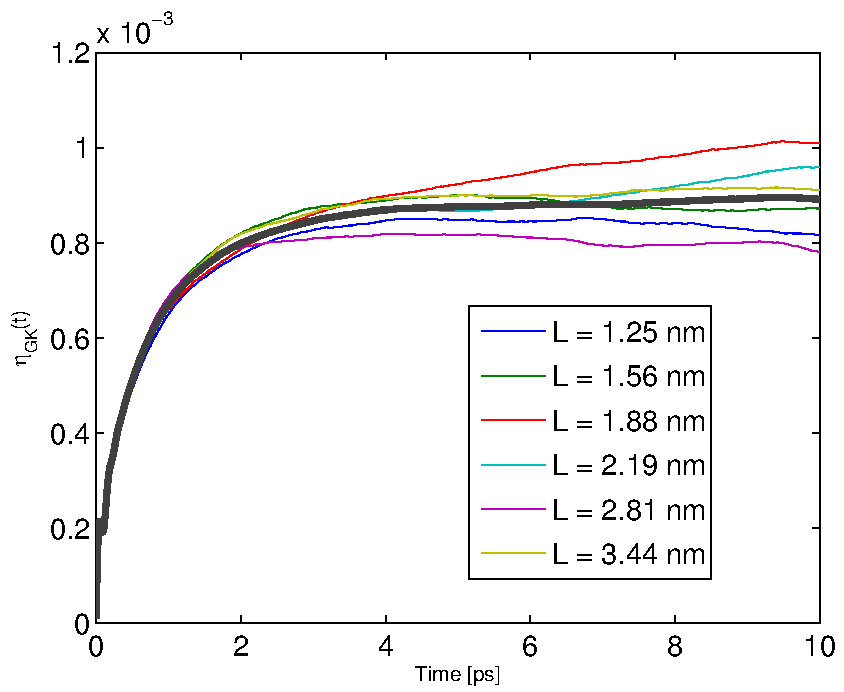
\includegraphics[width=10cm]{../figures/thesis/viscosity_green_kubo_tip4p_2005.pdf}
\caption{Shear viscosity for TIP4P/2005 at \SI{300}{\kelvin} and $\rho = \text{\SI{0.98}{\gram\per\cubic\cm}}$. The viscosity is estimated to $\eta_{GK} = \text{\SI{0.89\pm0.03}{\milli\pascal\second}}$. Note the little bump all to the left in the plot, which corresponds to a little period of negative values of the autocorrelation function. Seeing this little bump verifies that the time resolution of the measurement is sufficiently fine.}
\label{fig:shear_viscosity_tip4p/2005}
\end{figure}

In principle, the same simulation can be used to calculate the diffusivity, using the einstein relation \ref{eq:Einstein_diffusivity}. But long simulations are not the way to go when estimating diffusion. An average over several shorter simulations, around \SI{300}{\pico\second}, gives better estimates. 
In Figure \ref{fig:diffusivity_tip4p_2005} I use a weighted linear regression on the diffusion coefficient for different system lengths. As mentioned in the theory section, the diffusion coefficient in a periodic molecular dynamics system depend on the box size, and this finite size effect on it goes like $L^{-1}$. Underlying each (red) data point in Figure \ref{fig:diffusivity_tip4p_2005} are $N_s(L)=9$ simulations of \SI{320}{\femto\second}. Each of these simulations contribute an estimate of the diffusion coefficient using the Einstein relation on the mean squared displacement, and the mean of these $N_s(L)$ estimates is plotted. Error bars are estimated using the standard deviation of the $N_s(L)$ estimates: 
\begin{equation}
	e(L) = \sqrt{\frac{\text{var}(D(L))}{N_s(L)}}
\end{equation}
The expectation vaule of this error should go like $e \propto L^{-3/2}$ (inverse of the square root of the number of particles), which could have been another way to determine the weights.
Then, the regression line is found with weighted linear regression where the weights are:
\begin{equation}
	w(L) = \frac{1}{e(L)^2}
\end{equation}

Using this procedure, I estimate the diffusivity in the TIP4P/2005 model at $T=\SI{300}{\kelvin}$ and $\rho = \SI{0.98}{\gram\per\centi\meter\cubed}$ to $D_0=\text{\SI{2.46\pm0.07d-9}{\meter\squared\per\second}}$, which agrees well with the reference value. For completeness, Figure \ref{fig:msq_tip4p_2005} contains the data underlying the diffusion coefficient calculations. It is included to show how noisy the data are -- the model verification would not be satisfactory with just one simulation for each length of the simulation box.

\begin{figure}
\centering
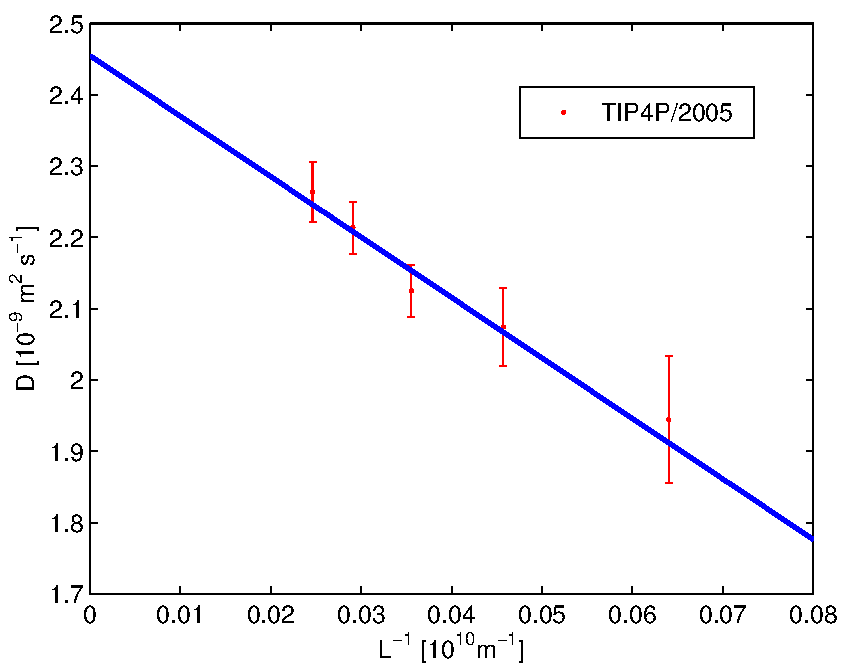
\includegraphics[width=10cm]{../figures/thesis/diffusion_coefficient_tip4p_2005.pdf}
\caption{Diffusivity for TIP4P/2005 for simulations with the same conditions as in Figure \ref{fig:shear_viscosity_tip4p/2005}. The diffusivity is estimated to $D_0=\text{\SI{2.46\pm0.07d-9}{\meter\squared\per\second}}$.}
\label{fig:diffusivity_tip4p_2005}
\end{figure}

\begin{figure}
\centering
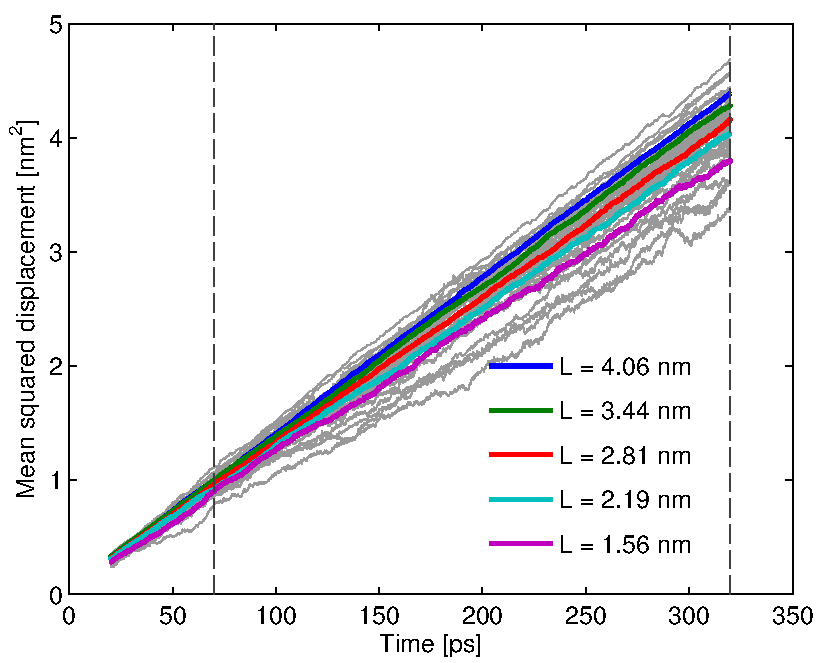
\includegraphics[width=10cm]{../figures/thesis/msq_tip4p_2005.pdf}
\caption{The data underlying Figure \ref{fig:diffusivity_tip4p_2005} (grey, thin lines) and the mean squared displacement averaged over $N_s$ simulation for each system length $L$ (colored, thick lines). Dashed vertical lines indicate the timeframe over which the diffusion coefficient was estimated.}
\label{fig:msq_tip4p_2005}
\end{figure}

Having measured both the shear viscosity and the diffusivity well within the uncertainty of reference values, I trust that my input files for the water model are correct, and go on to checking the methane model.

\section{United atom methane}
The methane model is simply a Lennard-Jones model, and I will use it with a sutoff and no long-range corrections. Young's modulus and Poissons ratio for the Lennard-Jones model will be verified when I check my protocol for measuring elastic properties in molecular dynamics. I an confident that LAMMPS treats the Lennard-Jones potential correctly, and I will have confirmation that my parameter input is correct if Young's modulus is correct (which it turns out to be).

\section{Stabilizing methane hydrates}
The TIP4P/ICE potential should be able to stabilize a methane hydrate stucture. Therefore, I prepared an S1 hydrate using positions priovided by \citet{Takeuchi2013}. These positions were derived using the TIP4P (no suffix) potential, and are not expected to be an equilibrium configuration for TIP4P/ICE. The hydrate turns out to equilibrate nicely – although some water molecules turn around – using a Nosé-Hoover NPT thermostat with a temperature rising from $0$ to \SI{30}{\kelvin}. The reason for using a rising temperature rather than an energy minimization, is that the energy minimization schemes don't work with the SHAKE-algorithm in LAMMPS, as discussed in section \ref{sec:shake} about the SETTLE algorithm.

\begin{figure}
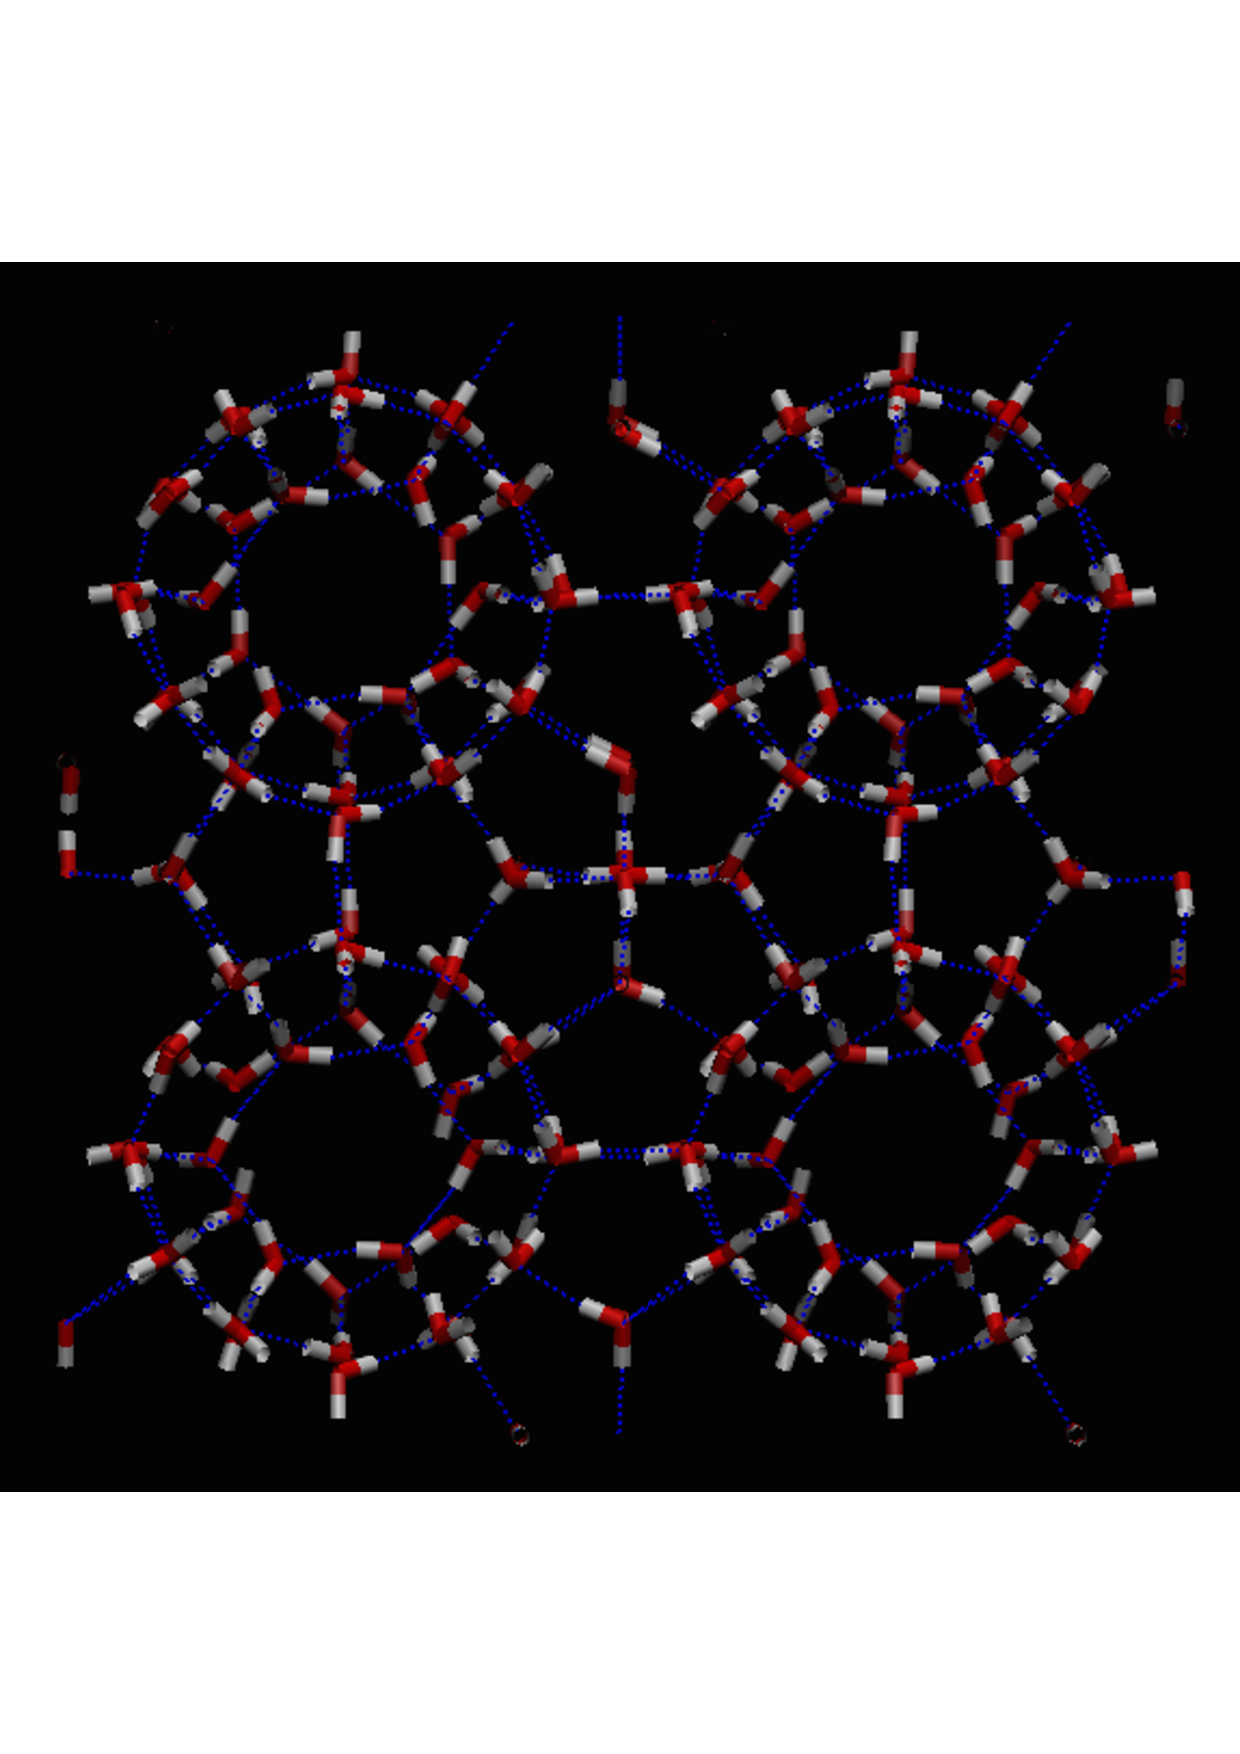
\includegraphics[width=\textwidth]{../snapshots/first_stable_hydrate.pdf}
\caption{Methane hydrate at low temperature. Rendered with VMD}
\label{fig:part2:first_hydrate}
\end{figure}

\section{Three-phase equilibrium line for methane hydrate}
Three-phase equilibrium simulations have been performed to check whether the model system is in the same ballpark as systems from the literature. Simulations have been performed on a system similar to the one in \cite{Conde2010}.

\begin{comment}
\section{Nucleation of methane hydrates?}
Nucleation of methane hydrates in a solution of water and methane is a rare event, and microsectond-simulations are required. 
\end{comment}

\section{Numerical efficiency}
Increasing the number of processor cores running a simulation almost always mean each cpu will work less effectively on the numerical task. But the wall time goes down, which means human waiting time goes down. Human waiting time is not critical in this project, since the results won't be applied immidiately. Therefore, a reasonable balance between computational efficiency and human waiting time should be found. Figure \ref{fig:lammps_efficiency} shows the numerical efficiency of simulating a large system on up to 300 cpu cores.

\begin{figure}
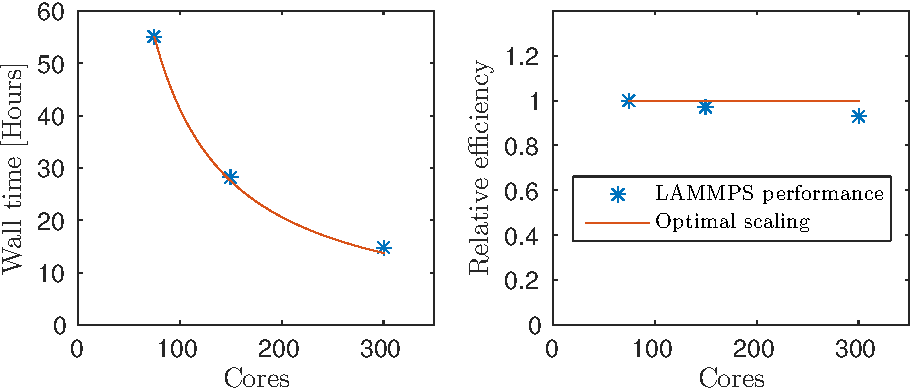
\includegraphics[width=\textwidth]{../figures/thesis/lammps_efficiency.pdf}
\caption{Wall time (left) and relative computational efficiency (right) for a sI methane hydrate system with approximately $10^6$ atoms.}
\label{fig:lammps_efficiency}
\end{figure}

\section{A subtle bug that took a lot of time to figure out -- Atoms out of range during P$^3$M calculation}

Since dealing with technical problems is a huge part of computational physics, I feel it necessary to describe some of the problems I have experienced. The most painful error that I experienced after getting rid of the beginners mistakes, was the following:

\begin{verbatim}
ERROR: Out of range atoms - cannot compute PPPM (../pppm_tip4p_omp.cpp:385)
\end{verbatim}

This is painful to debug. It typically shows up in large simulations after a long time, and with no clear reason. Molecular dynamics simulations expensive and time consuming, and each attempt on a solution to this problem typically requires hours even on a supercomputer. 

LAMMPS defaults to reduilding neighbor lists every 10 timesteps. In some cases this is not sufficient when using TIP4P with PPPM, so the standard solution to this is to force more frequent neighbor list builds:

\begin{lstlisting}[language=LammpsInput]
neigh_modify delay 0 every 1 check yes
\end{lstlisting}

However, this did not help me when i got the message. The next thing I tried was to half the timestep, which did not work either.

The next approach is to try to increase the damping time of the thermostat, as thermostats with a low characteristic time are known to cause trouble. But this did not help eiter. Then I realized that I did not experience this problem when I did not change from NPT to NVT during the simulation. Something ugly may happen when this is done.

To avoid doing NPT and NVT in the same simulation, I can start by creating an equilibrated system containing a crack, and use the simulation box size and particle positions from that simulation as input in my crack simulations. This of course also introduces the advantage of not having to equilibrate the system for every simulation. However, it also introduces the disadvantage of needing a separate file for each initial crack size.

It turned out that the problem was related to the OpenMP package bundled with LAMMPS. Some bug is introduced when using NPT and the OpenMP package. The OpenMP package did not give vital efficiency imporvements, so I choose not to use the OpenMP package rather than resolving the error.

There are signatures of this error in the total energy curve of the system. Figure \ref{fig:toteng_omp_bug} shows the total energy of an sI system while waiting for a crack to propagate. The simulation failed with the error message described above. As indicated in the figure, small discontinuities can be spotted in the total energy curve. For this particular simulation, there was also a large spike close to the end of the simulation, but that kind of spike doesn't show up often.

\begin{figure}
\centering
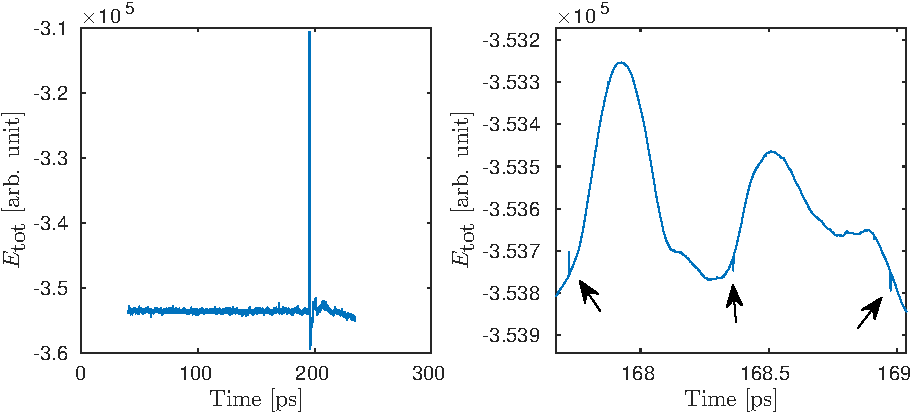
\includegraphics[width=\textwidth]{../figures/thesis/toteng_omp_bug.pdf}
\caption{Little spikes (indicated with arrows) in the total energy curve hint that someting is wrong with the simulation. These spikes disappeared when I stopped using the USER-OMP package. Note the small time-window in the right panel. These spikes are only visible when zooming closely in on the data.}
\label{fig:toteng_omp_bug}
\end{figure}
